% -------------------------------------------------------------------------
\subsubsection{File Format for Individual Objects}
\label{grammar}

We describe the individual objects in the following table. The first
column lists the non-terminal symbol. The second column lists grammar
rules where several alternative choices are listed below each other.
The third column gives a description of the object.  Non-terminal
symbols formatted in boldface are valid \nts{Object} entries that can
follow the classification. The other non-boldface non-terminal symbols
are only used within the grammar rules of other symbols.  The non-bold
objects are auxiliary tokens that occur only in the structure of bold
objects. \medskip

\begin{tabular}{*{3}{| l} |} \hline
Object   & syntax                         & description \\ \hline \hline
Integer  & INTEGER                        & an integer value \\ \hline
Rational & Rational (Integer, Integer)    & Rational(integer nominator, \\
         &                                & \ \ \ \ \ \ \ \ \ \ \ \ \ integer denominator)
                                            \\ \hline
Infty    & MINUS\_INFTY                   & encodes $-\infty$ \\ 
         & PLUS\_INFTY                    & encodes $+\infty$  \\ \hline

Integer\_sequence & integer\_sequence (Integer,...)      
                        & a sequence of arbitrary many integer  \\ 
                  &     &  values \\ \hline
%Integer\_sequence\_2 & integer\_sequence\_2(
%                       & a sequence of an even number of \\
%                  & \ \ Integer, Integer, ... ) & integer values\\ \hline
Orientation & COUNTERCLOCKWISE            & orientation of a ConicArc  \\
            & CLOCKWISE                   &           \\
            & VOID                        &           \\ \hline

Point\_2 & Point\_2 (Integer,Integer)     & cartesian point with \\
         &                                & \ \ integer coordinates x and y \\
         & Point\_2 (Integer,Integer,Integer) & homogeneous point with \\ 
         &                                & \ \ integer coordinates x,y,w\\
         & Point\_2 (Rational,Rational)   & cartesian point of two \\
         &                                & \ \ rational coordinates x,y\\ \hline
%InterpolationPoint & InterpolationPoint\_2 (   & an InterpolationPoint consits 
%                                                  of a point \\
%                   & \ \ Point\_2 ,            & and its derivations\\
%                   & \ \ Integer\_sequence\_2 )&  \\ \hline
{\bf Polynomial}    & {\bf Polynomial\_1} (Integer\_sequence) 
                             & the coefficients of an integer polynomial \\ \hline

AlgebraicReal & AlgebraicReal (         & an algebraic real is a real root\\
              & \ \ Polynomial,         & of a polynomial defined by an\\
              & \ \ Rational,Rational,  & isolating interval with rational boundaries\\
              & \ \ Integer)            & or redundantly by the index of the root\\ \hline

{\bf LineSegment} & {\bf LineSegment\_2} (Point\_2,Point\_2) & LineSegment\_2 (source, target) \\ \hline

{\bf Circle}   & {\bf Circle\_2} (Point\_2,Integer) & Circle\_2 (center, radius) \\ 
               & {\bf Circle\_2} (Point\_2,Rational) & Circle\_2 (center, radius) \\ \hline

{\bf Conic}  & {\bf Conic\_2} (
                               & Conic defined by its 6 coefficients \\
             & \ \ \ \ \ Integer,Integer,Integer,
                     &  (A,B,C,D,E,F) \\
             & \ \ \ \ \ Integer,Integer,Integer)        
                     &  \begin{math} Ax^2+Bxy+Cy^2+Dx+Ey+F \end{math}\\ \hline

%{\bf InterpolatedConic} & {\bf InterpolatedConic} (   
%                                            & consits of a nonempty sequence \\
%                 & \ \ Interpolation\_point\_2\_sequence ) 
%                                            & of InterpolationPoints\\ 
%                  &                         & 5 interpolation conditions 
%                                                    are necessary\\ 
%                  &                         & for a conic \\ \hline

ConicPoint    & ConicPoint\_2 (Conic,  
                        & ConicPoint (Conic, x-coordinate, \\
              & \ \ AlgebraicReal,Integer)  
                        & \ \ arc number implying y-coordinate (0 or 1)) \\
              & ConicPoint\_2 (Conic,          
                        & ConicPoint (Conic, x-coordinate at infinity, \\
              & \ \ infty,Integer) 
                        & \ \ arc number) \\
              & ConicPoint\_2 (Conic,    
                        & ConicPoint (Conic, x-coordinate, \\
              & \ \ AlgebraicReal,infty) 
                        & \ \ y-coordinate at infinity) \\ \hline
%              & ConicPoint\_2 (InterpolatedConic,  
%                       & ConicPoint (Conic, y-coordinate, \\
%              & \ \ AlgebraicReal, Integer)  
%                        & \ \ x-coordinate) \\
%              & ConicPoint\_2 (InterpolatedConic,    
%                      & ConicPoint (Conic, y-coordinate, \\
%              & \ \ AlgebraicReal, infty) 
%                    & \ \ x-coordinate) \\
%              & ConicPoint\_2 (InterpolatedConic,          
%                  & ConicPoint (Conic, y-coordinate, \\
%              & \ \ infty, Integer) & \ \ x-coordinate) \\ \hline



{\bf ConicArc}      & {\bf ConicArc\_2} (Conic,    & an Arc of a Conic \\
              & \ \ ConicPoint,                    & with source,\\
              & \ \ ConicPoint,                    & target, and\\
              & \ \ Orientation)                   & its orientation\\
%              & {\bf ConicArc\_2} ( InterpolatedConic,    & \\
%              & \ \ ConicPoint,                    & \\
%              & \ \ ConicPoint,                    & \\
%              & \ \ orientation)                   & \\               
              & {\bf ConicArc\_2} (ConicPoint)      & degenerated arc (single point) \\ \hline


{\bf Cubic} & {\bf Cubic\_2} (        & Cubic defined by its 10 coefficients \\
      & \ \ Integer, Integer, Integer & (A,B,C,D,E,F,G,H,K,L)\\
      & \ \ Integer, Integer, Integer & \begin{math} Ax^3+Bx^2y+Cxy^2+Dy^3+Ex^2+ \end{math}\\
      & \ \ Integer, Integer, Integer & \begin{math}Fxy+Gy^2+Hx+Ky+L\end{math}\\
      & \ \ Integer)                  & \\ \hline

%{\bf InterpolatedCubic} & {\bf InterpolatedCubic\_2} (   & \\
%                  & \ \  Interpolation\_point\_2\_sequence ) & \\ \hline
{\bf Quadric} & {\bf Quadric\_3} (      & Quadric defined by its 10 coefficients \\
        & \ \ Integer, Integer, Integer & (A,B,C,D,E,F,G,H,K,L)\\
        & \ \ Integer, Integer, Integer & \begin{math} Ax^2+Bxy+Cxz+Dy^2+Eyz+ \end{math}\\
        & \ \ Integer, Integer, Integer & \begin{math}Fz^2+Gx+Hy+Kz+L\end{math}\\
        & \ \ Integer)                  & \\ \hline

\end{tabular}

\subsubsection {Example: Complete File for Conics}
\label{longexample}

\begin{figure}
  \centerline{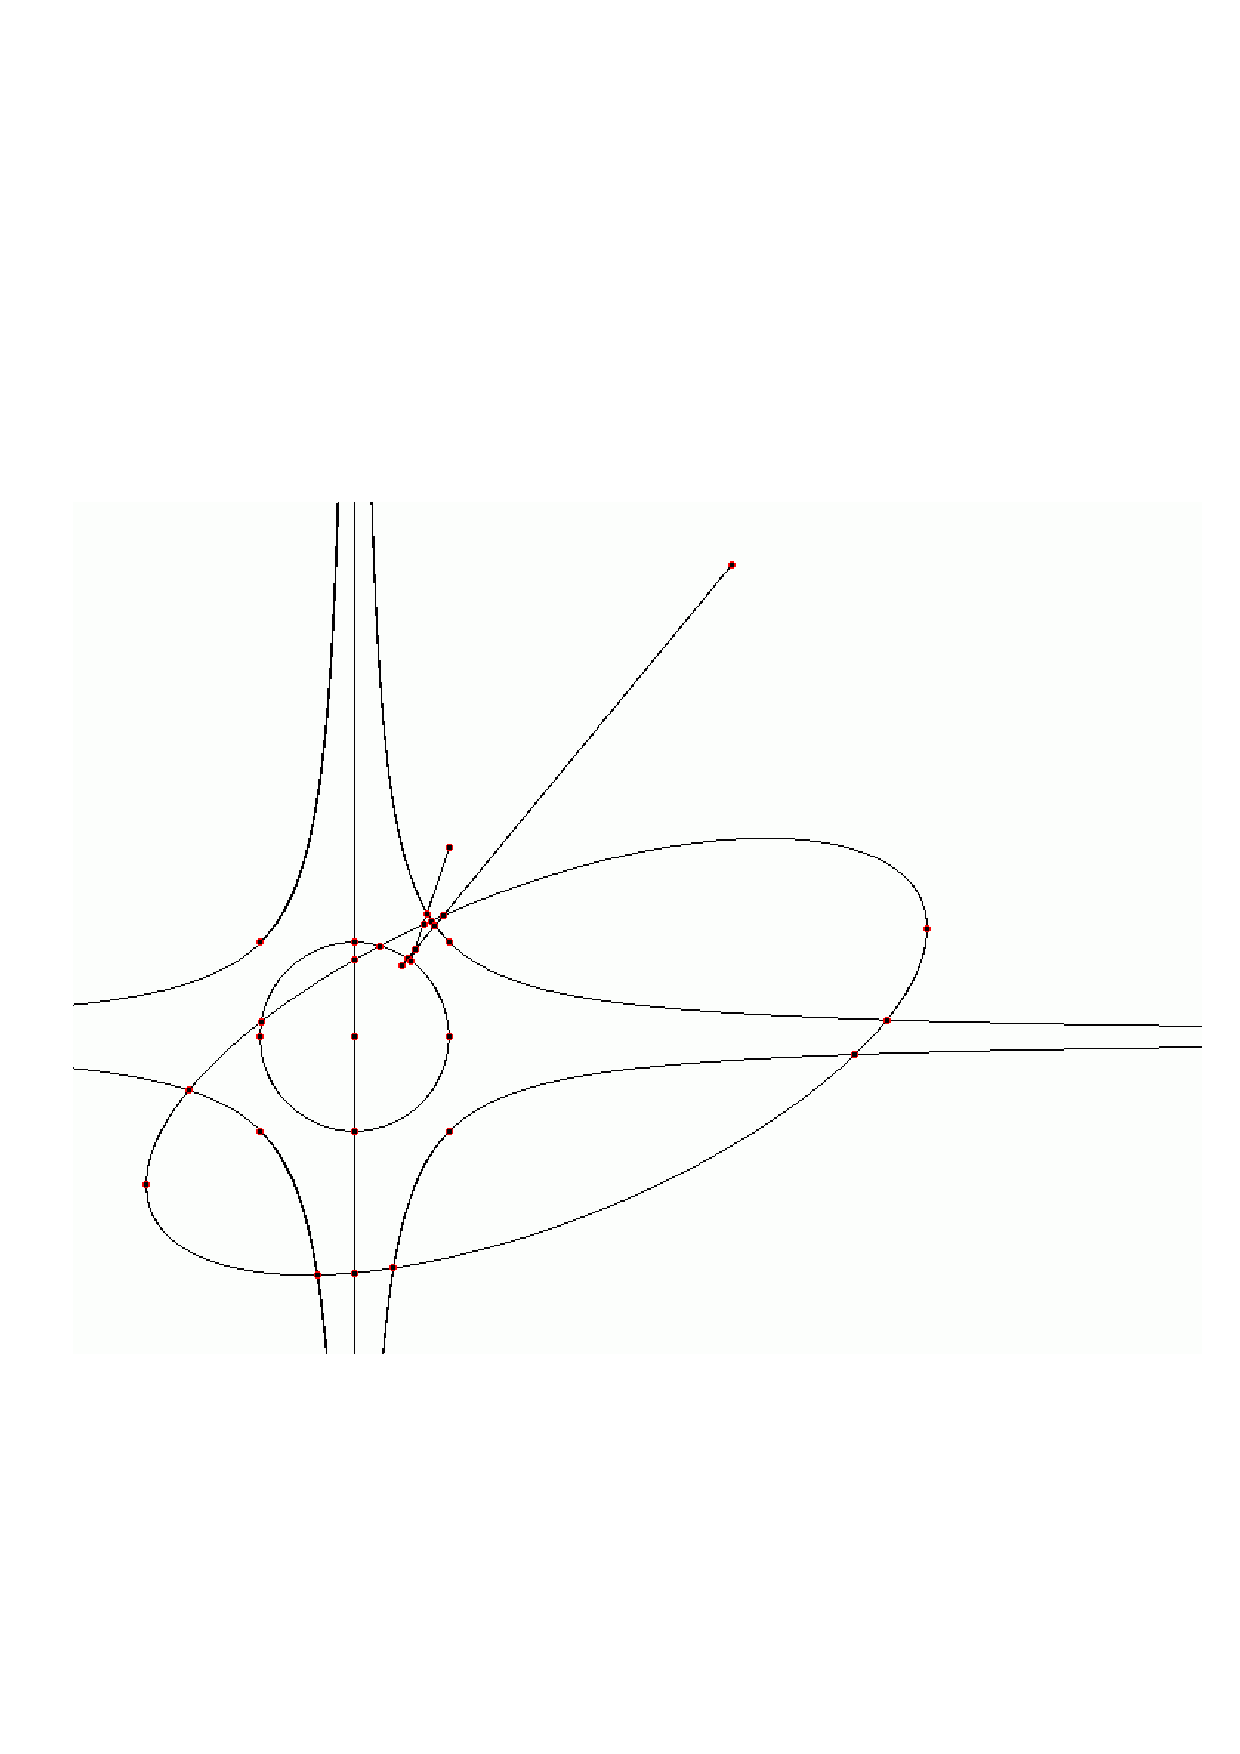
\includegraphics[width=0.7\textwidth]{Benchmark/fig/Conics_14_1}}

  \caption{The curves and arcs contained in the example benchmark
    file.\label{fig:example}}
\end{figure}

We give a longer example containing 14 object of different types; line
segments, circles, conics, bounded and unbounded arcs of conics. See
Figure~\ref{fig:example} for their geometry.

% \IncludeVerbatim{Benchmark/Conics_14_1.arr}
\ccIncludeExampleCode{Benchmark/Conics_14_1.arr}
